\documentclass[%
        %draft,
        %submission,
        %compressed,
        final,
        %
        %technote,
        %internal,
        %submitted,
        %inpress,
        %reprint,
        %
        %titlepage,
        notitlepage,
        %anonymous,
        narroweqnarray,
        inline,
        %twoside,
        ]{ieee}
%
% some standard modes are:
%
% \documentclass[draft,narroweqnarray,inline]{ieee}
% \documentclass[submission,anonymous,narroweqnarray,inline]{ieee}
% \documentclass[final,narroweqnarray,inline]{ieee}

\usepackage{ieeefig,url,enumerate}

\begin{document}

\title{Scaling Machine Learning Algorithms}

% format author this way for journal articles.
\author[SHORT NAMES]{
  Juan Batiz-Benet \\
  \and{\quad\quad}
  Quinn Slack \\
  \and{\quad\quad}
  Matt Sparks \\
  \and{\quad\quad}
  Ali Yahya
}

% specifiy the journal name
%\journal{IEEE Transactions on Something, 1997}

% Or, when the paper is a preprint, try this...
%\journal{IEEE Transactions on Something, 1997, TN\#9999.}

% Or, specify the conference place and date.
%\confplacedate{Ottawa, Canada, May 19--21, 1997}

\maketitle

\begin{abstract}
We wish to provide a portable framework for the rapid prototyping of machine
learning algorithms on a cluster of computers.
\end{abstract}

% do the keywords
%\begin{keywords}
%keyword 1, keyword 2 ...
%\end{keywords}

\section{Introduction}

% try out a theorem...
\newtheorem{theorem}{Theorem}

\begin{theorem}[Theorem name]
  Consider the system ...
\end{theorem}

\begin{proof}
  The proof is trivial.
\end{proof}

\section{Distributing Work}

In order for an algorithm to be run in parallel on several machines, some part
of it must be amenable to parallelization. More specifically, some component or
step of the algorithm must be able to be subdivided into \emph{workunits} that
can be processed in parallel by multiple nodes with little or no communication
between the nodes. If communication between nodes is excessive, the overhead of
distributing the work becomes dominant and the any potential performance gained
by running in parallel is lost.

More here about batch gradient descent as an example algorithm that can be
easily distributed.

\section{Rapid Prototyping}

Previous work has been done in distributing Matlab. However, due to licensing
constraints, this is not feasible for large clusters. We needed to choose
another environment in which to develop and test machine learning
algorithms. For this project, we considered Python and R as alternatives to
Matlab.

\subsection{Requirements}

Words here about why R and Python might be good choices. (Packages available
for matrix manipulations, highly general, free, easy to pick up and use,
portable?)

\subsection{Benchmarks}

Benchmark data for Python vs R (vs Matlab?)

Perhaps also some words here about why Python is still acceptable even if it is
significantly slower than Matlab. In particular, we are doing rapid
prototyping, so peak CPU performance isn't the deciding factor. We are more
interested in processing lots of data by distributing it to enough nodes such
that the data can fit in memory and be processed effectively.

\section{Framework Design}

\subsection{Conventional Approaches}

Some words here about how the batch gradient descent example easily lends
itself to a straight mapreduce workflow. Because of this workflow, we first
considered using an existing mapreduce framework for our project.

One such framework we considered is Hadoop MapReduce. Some words here about why
Hadoop doesn't apply well to our problem. Consider the batch gradient decent
example again. Each iteration is essentially a mapreduce operation: the
examples are split up and distributed, the individual sums are calculated at
each node, and the reduce operation is calculating the final sum. The examples
considered at each node must remain stored locally at that node, ideally in
memory, for later recall during the next mapreduce operation for the subsequent
iteration.

Some words here about Disco and its attempt to solve this problem?

\subsection{Our design}

Our design consists of a single master and one or more slaves, as shown in
Fig. \ref{diagram}.

\begin{figure}[hb]
  \begin{center}
    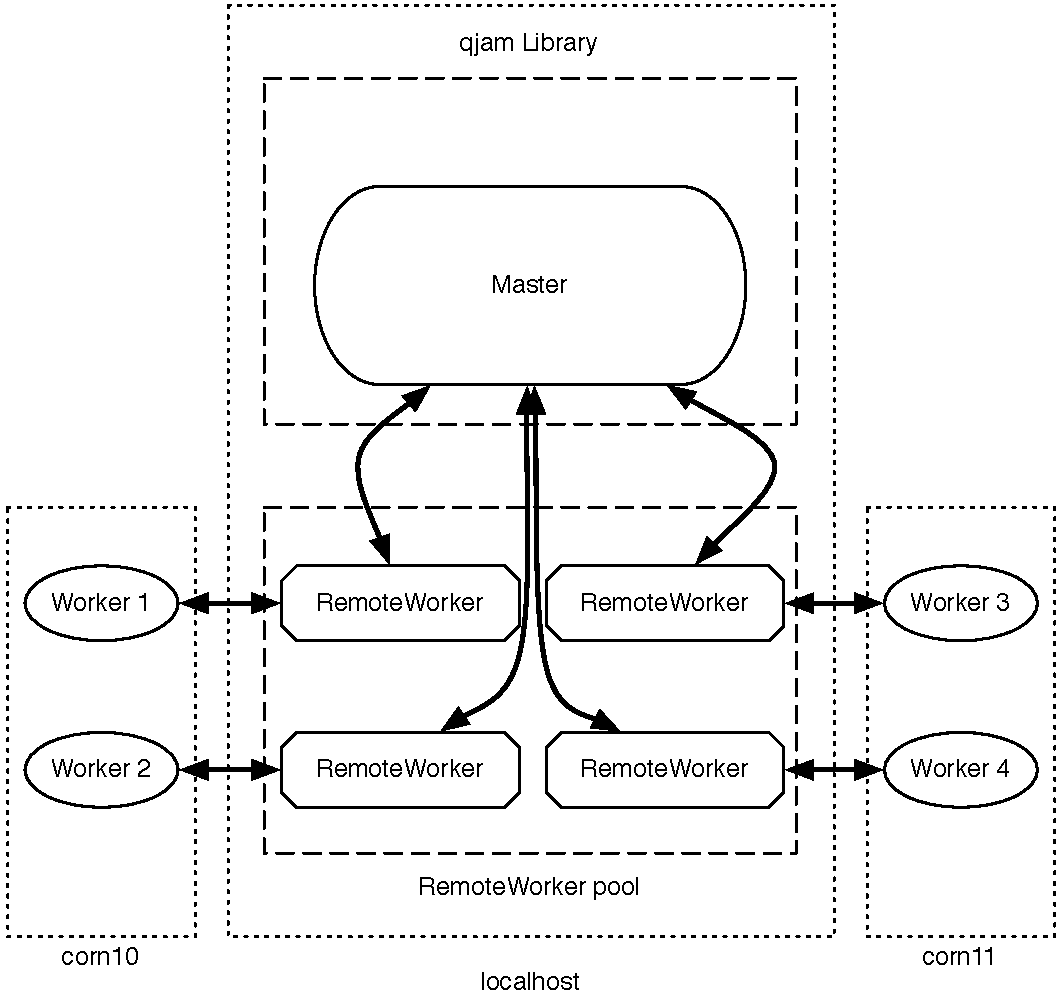
\includegraphics[width=2.5in]{fwk_diagram/fwk_diagram.pdf}
  \end{center}
  \caption{Diagram of our framework.}
  \label{diagram}
\end{figure}

First, on the master, you define a Python map function with the following prototype:
\begin{verbatim}
    def mymap(examples, params):
        psum = 0
        for (xi,yi) in examples:
            psum += (yi - g(params.theta.T * xi)) * xi
        return psum
\end{verbatim}

Then, also on the master, you specify your training examples and initial parameters:
\begin{verbatim}
    examples = ((x1, y1), (x2, y2), (x3, y3))
    params   = (0, 0, 0)
\end{verbatim}

The difference between examples and parameters is that examples will not be
resent on each iteration. We will check whether the slave already has the {\tt
  examples} object (with the same hash) and only resend it if needed. The
parameters data, however, will be resent for each iteration. These two objects
can be arbitrarily typed, as long as they are serializable. For example, for
large datasets, we might implement a list/dictionary proxy (that behaves like
its standard Python counterpart but doesn't store everything in memory). Also,
typically they will hold {\tt numpy} arrays and matrices instead of Python
tuples as shown in the example above.

To start the job, call:

\begin{verbatim}
    master.run(mymap, examples, params)
\end{verbatim}

This instructs the master to serialize the map function, training data, and
initial parameters, and send them to the slaves, each of which is listening for
jobs. Each slave will run the {\tt mymap} function, with the parameters in {\tt
  params} and some portion of the training set available in {\tt examples}.

This call will block until all slaves respond with their partial sums. The {\tt
  run} method will apply the {\tt sum} reduce function to each slave's response
and will return the total sum. (For easy local testing, the {\tt mymap}
function can also be run on the local machine in the same Python process.)

We will initially ignore slave failures. Failure tolerance can be added
later (reship the local data, rerun dead slave's work). The master shares its fate
with the main program being run; if the main program dies, the master dies with
it, and vice versa. Thus, we do not need replicated masters or anything
similarly sophisticated.

\subsection{Serialization and Slave-Local Storage}

We initially aim to support training sets around 30 GB, so we must have a way
to distribute this data to the nodes without having to send it to each node for
each iteration. In the MapReduce model, {\tt map} function only relies on data
given to it; there is no global data. This lets the master control distribution
of the data using its superior knowledge about the cluster size and
capabilities, and it reduces data transmission overhead.

When the master runs a job on $n$ slaves, it creates $n$ equal slices of the
training set and assigns one to each slave. On subsequent iterations, each
slave will be assigned the same data slice, as long as no slaves join or leave
the cluster. The master then sends the data slice to the slave, but only if the
slave doesn't already have the data.

We expect that the initial serialization and transmission of the training set
to each slave will take quite a while. This is an area ripe for future
optimization. However, we won't naively succumb to the vice of premature
optimization unless this is a major bottleneck.

Each slave will know what data slice it has, and will use that data slice as
arguments to the {\tt map} function.

This is similar to the SlaveRefs in Adam Coates' Matlab parallel framework, but
we are able to use Python's superior syntax to hide the implementation details
of references to data on slaves. Also, our system as described will only send
portions of the data to each slave, which will decrease data transmission
overhead.

% do the biliography:
%\bibliographystyle{IEEEbib}
%\bibliography{my-bibliography-file}

%----------------------------------------------------------------------
% FIGURES
%----------------------------------------------------------------------
% There are many ways to include figures in the text. We will assume
% that the figure is some sort of EPS file.
%
% The outdated packages epsfig and psfig allow you to insert figures
% like: \psfig{filename.eps} These should really be done now using the
% \includegraphics{filename.eps} command.
%
% i.e.,
%
% \includegraphics{file.eps}
%
% whenever you want to include the EPS file 'file.eps'. There are many
% options for the includegraphics command, and are outlined in the
% on-line documentation for the "graphics bundle". Using the options,
% you can specify the height, total height (height+depth), width, scale,
% angle, origin, bounding box "bb",view port, and can trim from around
% the sides of the figure. You can also force LaTeX to clip the EPS file
% to the bounding box in the file. I find that I often use the scale,
% trim and clip commands.
%
% \includegraphics[scale=0.6,trim=0 0 0 0,clip=]{file.eps}
%
% which magnifies the graphics by 0.6 (If I create a graphics for an
% overhead projector transparency, I find that a magnification of 0.6
% makes it look much better in a paper), trims 0 points off
% of the left, bottom, right and top, and clips the graphics. If the
% trim numbers are negative, space is added around the figure. This can
% be useful to help center the graphics, if the EPS file bounding box is
% not quite right.
%
% To center the graphics,
%
% \begin{center}
% \includegraphics...
% \end{center}
%
% I have not yet written good documentation for this, but another
% package which helps in figure management is the package ieeefig.sty,
% available at: http://www-isl.stanford.edu/people/glp/ieee.shtml
% Specify:
%
%\usepackage{ieeefig}
%
% in the preamble, and whenever you want a figure,
%
%\figdef{filename}
%
% where, filename.tex is a LaTeX file which defines what the figure is.
% It may be as simple as
%
% \inserteps{filename.eps}
%
% or
% \inserteps[includegraphics options]{filename.eps}
%
% or may be a very complicated LaTeX file.

\end{document}
